\chapter{Methodology}

\section{Project Approach}
TPMS is a product-based software engineering project developed following a \textbf{Prototyping-driven Iterative Development Approach}. This methodology was chosen because academic workflows at DOECE involve domain-specific rules, such as multi-tier marking schemes, student team constraints, and supervisor-examiner allocations, that required progressive refinement and validation with departmental stakeholders.

The project execution was organized into four structured phases:
\begin{itemize}
  \item \textbf{Phase 1: Requirement Analysis and Design (Weeks 1--3):} Departmental requirement gathering, entity-relationship modeling, database schema design, and interactive UI wireframing.
  
  \item \textbf{Phase 2: Core Authentication and Workflow Management (Weeks 4--7):} Implementation of Role-Based Access Control (RBAC), user authentication, student group registration, proposal submissions, and coordinator management views.
  
  \item \textbf{Phase 3: Evaluation Engine and Document Generation (Weeks 8--11):} Development of criteria-wise defense scoring interfaces, automated mark calculation algorithms, and server-side print-ready A4 PDF evaluation sheet generation.
  
  \item \textbf{Phase 4: Bulk Data Ingestion, Notifications, and Testing (Weeks 12--14):} Implementation of spreadsheet roster onboarding, email notification workers, functional system testing, user feedback incorporation, and final report compilation.
\end{itemize}

\section{System Architecture}
TPMS is designed following a \textbf{three-tier client-server architecture} that enforces a strict separation of concerns among the presentation, application logic, and data persistence layers \cite{martin2017clean}. This decoupled design ensures system maintainability, modularity, and security.

Figure~\ref{fig:arch} illustrates the high-level layered architecture of the system:

\begin{enumerate}
  \item \textbf{Presentation Layer (Frontend Tier):}  
  The top tier consists of a modern Single-Page Application (SPA) accessible via standard web browsers. It provides dedicated, role-specific dashboards tailored for Students, Supervisors, External Examiners, Program Coordinators, and Department Maintainers. This layer manages dynamic user interactions, client-side input validations, visual state updates, and communicates asynchronously with the backend server through standard REST API requests.

  \item \textbf{Application Logic Layer (Backend Tier):}  
  The middle tier serves as the core processing engine of the system. It handles API routing, user authentication and JWT verification, Role-Based Access Control (RBAC) enforcement, business rule validation, and defense mark computations. Additionally, this layer executes background tasks, including the generation of university-standard A4 PDF evaluation scorecards and the dispatch of automated email notifications.

  \item \textbf{Data Persistence Layer (Database Tier):}  
  The bottom tier comprises a relational PostgreSQL database managed through an Object-Relational Mapping (ORM) layer. It securely stores normalized relational data, including user credentials, student cohorts, project group structures, proposal manuscripts, supervisor allocations, and defense mark ledgers, ensuring ACID compliance and strong referential integrity across all records.
\end{enumerate}

\begin{figure}[H]
\centering
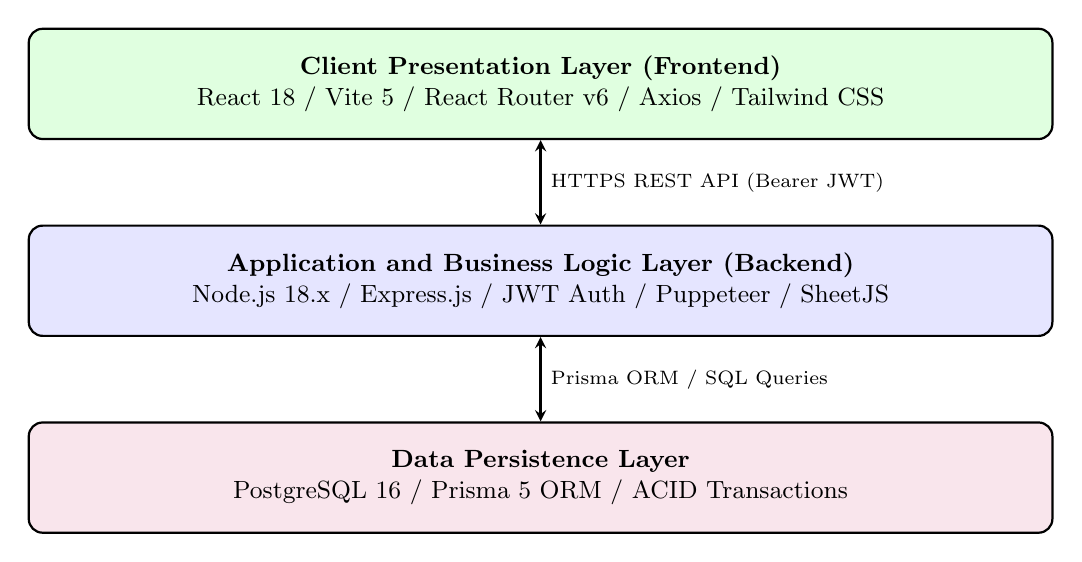
\begin{tikzpicture}[
  layer/.style={draw, thick, rounded corners=5pt,
    minimum width=13cm, minimum height=1.4cm,
    align=center, font=\small},
  arr/.style={thick, <->, >=stealth}
]
\node[layer, fill=green!12] (fe) at (0, 0)
    {\textbf{Client Presentation Layer (Frontend)}\\
     React 18 / Vite 5 / React Router v6 / Axios / Tailwind CSS};

\node[layer, fill=blue!10] (be) at (0,-2.5)
    {\textbf{Application and Business Logic Layer (Backend)}\\
     Node.js 18.x / Express.js / JWT Auth / Puppeteer / SheetJS};

\node[layer, fill=purple!10] (db) at (0,-5.0)
    {\textbf{Data Persistence Layer}\\
     PostgreSQL 16 / Prisma 5 ORM / ACID Transactions};

\draw[arr] (fe) -- node[right,font=\scriptsize]{HTTPS REST API (Bearer JWT)} (be);
\draw[arr] (be) -- node[right,font=\scriptsize]{Prisma ORM / SQL Queries} (db);
\end{tikzpicture}
\caption{Three-Tier System Architecture of TPMS}
\label{fig:arch}
\end{figure}

\section{System Design and Modules}
To ensure maintainability, scalability, and clean separation of concerns, TPMS is structured into cohesive functional modules. Each module encapsulates specific business logic and provides defined interfaces for user interaction and data processing:

\subsection{Authentication and Access Control Module}
This module manages secure user authentication and authorization across the platform. It handles user login, password hashing using modern cryptographic standards, stateless JSON Web Token (JWT) issuance and verification, and role-based route protection. The module enforces the five-role hierarchy (Student, Supervisor, External Examiner, Program Coordinator, and Maintainer) and ensures program-scoped data isolation between undergraduate and graduate departments.

\subsection{Group Formation and Project Registration Module}
This module governs the initiation of the project lifecycle. Coordinators publish academic project announcements with defined deadlines and team size constraints. Undergraduate students use this module to create project groups, send peer invitations via university roll numbers, and submit project proposals and research cluster choices. For graduate programs, it facilitates individual thesis topic and proposal registration.

\subsection{Coordinator Management and Faculty Allocation Module}
This module provides department coordinators with a centralized dashboard to manage submissions in real time. It features a deduplicated response matrix displaying complete team rosters, proposal details, and research domains. Coordinators use this module to assign supervisors, designate external defense examiners, and enforce conflict-of-interest rules that prevent faculty from examining projects they supervise.

\subsection{Document and Submission Management Module}
This module provides structured document handling for all project deliverables throughout the semester. It enables students to upload proposal manuscripts, mid-term progress reports, and final thesis documents. Supervisors and coordinators can review submissions, provide actionable feedback, and track submission statuses without relying on scattered physical copies or email attachments.

\subsection{Evaluation and Mark Calculation Module}
This module implements the official departmental grading rubrics for Minor projects (50 marks), Major projects (100 marks), and Master theses (300 marks). It provides an interactive criteria-wise mark entry interface for supervisors and examiners. The module automatically computes total marks, enforces maximum score boundaries, converts numerical scores into words, and prevents unauthorized modification of finalized defense results.

\subsection{Automated Report and PDF Generation Module}
This module dynamically compiles database records into standardized, print-ready A4 PDF evaluation sheets conforming to official university formats. It supports single-group downloads as well as bulk multi-project exports, enabling coordinators to instantly generate complete evaluation packages for examination archives.

\subsection{Bulk Data Ingestion and Notification Module}
This module simplifies large-scale departmental administration through automated data onboarding and communication. It provides a spreadsheet import engine capable of validating student rosters, checking for duplicate entries, and batch-creating user accounts. In addition, an asynchronous notification worker dispatches automated email updates to students and faculty regarding supervisor allocations, feedback availability, and defense schedules.

\section{Technology Stack}
\begin{table}[H]
\centering
\caption{Technology Stack and Justification}
\label{tab:tech_stack}
\vspace{4pt}
\small
\begin{tabularx}{\textwidth}{@{}l p{4.2cm} X@{}}
\toprule
\textbf{Layer} & \textbf{Technology} & \textbf{Justification} \\
\midrule
Frontend       & React 18 / Vite 5       & Component-based SPA with fast build tooling and reactive rendering \\
               & React Router v6         & Client-side role-guarded routing and protected page views \\
               & Tailwind CSS            & Utility-first responsive styling and layout design \\
\midrule
Backend        & Node.js 18+ / Express.js & Non-blocking I/O runtime and modular HTTP REST API framework \\
               & Puppeteer Core          & Headless browser engine for server-side A4 PDF grade sheet compilation \\
               & SheetJS (xlsx)          & Spreadsheet parser for roster validation and bulk account creation \\
               & bcryptjs / jsonwebtoken & Cryptographic password hashing and stateless token management \\
               & Nodemailer              & SMTP mail transport client for automated email notifications \\
\midrule
Database       & PostgreSQL 16           & Enterprise-grade relational DBMS with ACID compliance \\
               & Prisma 5 ORM            & Type-safe database client with declarative schema migrations \\
\bottomrule
\end{tabularx}
\end{table}

\section{Development Methodology}
The project adopted the \textbf{Prototyping Model} to accommodate evolving departmental requirements and ensure close alignment with stakeholder expectations. The development workflow was carried out through the following structured stages:

\begin{itemize}
  \item \textbf{Requirement Elicitation and Analysis:} Functional and non-functional requirements were gathered through discussions with the project supervisor, program coordinators, and student peers to identify essential academic workflows and evaluation guidelines.
  
  \item \textbf{Prototype Design and Development:} Initial user interface wireframes and interactive mockups were created for core components, including role-based dashboards, proposal registration forms, and defense evaluation scorecards.
  
  \item \textbf{Stakeholder Evaluation and Feedback:} The preliminary prototypes were presented to the project supervisor and departmental coordinators for review, identifying workflow bottlenecks, UI improvements, and validation rules early in the process.
  
  \item \textbf{Iterative Refinement and System Implementation:} Feedback from review sessions was incorporated into successive development iterations, transitioning the prototypes into fully functional frontend interfaces connected to backend business logic and the database.
  
  \item \textbf{System Testing and Integration:} Completed modules underwent functional verification, data consistency checks, and user acceptance testing across simulated defense workflows to prepare the platform for deployment.
\end{itemize}

\section{Data Handling}
In the current implementation, all persistent system data and uploaded documents are stored and managed within the local server environment:

\begin{itemize}
  \item \textbf{Local Relational Database Storage:} All structured application records, including user credentials, role allocations, project group compositions, defense evaluations, and audit events, are persisted in a local PostgreSQL relational database managed via Prisma ORM. Queries are executed through parameterized statements, preventing SQL injection and maintaining strict relational integrity.
  
  \item \textbf{Local Filesystem Document Storage:} Uploaded project proposals, progress reports, and generated A4 PDF evaluation sheets are stored directly on the local server filesystem within a dedicated storage directory (\texttt{/storage}), categorized by degree program and academic cohort.
  
  \item \textbf{Input Validation and Sanitization:} Client inputs received through RESTful endpoints undergo server-side validation. Uploaded document files are restricted to PDF format and verified for size constraints before being written to local storage.
  
  \item \textbf{Password Security:} User passwords are encrypted using bcrypt with salt rounds before being stored in the database, ensuring that plaintext passwords are never recorded.
\end{itemize}

\section{Testing and Validation}
To ensure functional correctness, data integrity, and system reliability, testing was conducted across three distinct phases:

\begin{itemize}
  \item \textbf{Unit Testing:} Individual controller functions, authentication middleware, validation logic, and mark calculation algorithms were tested in isolation to verify correct output across standard and edge-case inputs.
  
  \item \textbf{Integration Testing:} End-to-end API workflows spanning multiple system modules, such as team creation, document submission, coordinator approval, defense mark tabulation, and PDF compilation, were tested to ensure seamless inter-module communication.
  
  \item \textbf{User Acceptance Testing (UAT):} Representative stakeholders, including program coordinators, faculty supervisors, and students, tested the system against structured task scenarios to evaluate user interface responsiveness, workflow clarity, and overall operational readiness.
\end{itemize}

\section{Deployment Setup}
The platform is fully configured and executed within a \textbf{local server deployment} for system evaluation and departmental demonstration:

\begin{itemize}
  \item \textbf{Local Application Servers:} The backend REST API service runs locally on Node.js (port 5000), while the React frontend application is served locally via the Vite server (port 5173).
  
  \item \textbf{Local Database Service:} A local PostgreSQL database instance (port 5432) hosts the application schemas and relations, with database migrations applied through the Prisma CLI.
  
  \item \textbf{Local File Management:} Document uploads and downloads are handled directly via Node.js file system streams accessing the local storage directory.
  
  \item \textbf{SMTP Email Integration:} Automated email notifications for milestone events, supervisor assignments, and defense feedback are dispatched through an integrated SMTP (Simple Mail Transfer Protocol) transport service, configured via local environment parameters.
  
  \item \textbf{Environment Security:} All local configurations, including database connection strings, JWT signing keys, and SMTP server credentials, are isolated in a root-level \texttt{.env} file.
\end{itemize}
